% Lecture Template for ME3001-001-Tristan Hill - Spring 2020
% Mechanical Engineering Analysis with MATLAB
% Ordinary Differential Equations - Lecture 2

% I am finally converting my stuff to BEAMER
% and I am putting these on Github because Dropbox is defective

% Document settings



%\documentclass{beamer}                  % for presentation ?
\documentclass[handout]{beamer}  % for handout ?
\usepackage{beamerthemesplit}
\usepackage{amsmath}
\usepackage{listings}
\usepackage{multicol}
\usepackage{framed}

\usepackage{soul}


\beamertemplateballitem

\definecolor{TTUpurple}{rgb}{0.3098, 0.1607, 0.5176} % TTU Purple (primary)
\definecolor{TTUgold}{rgb}{1.0000, 0.8666, 0.0000} % TTU Gold (primary)

\setbeamercolor{palette primary}{bg=TTUpurple,fg=TTUgold}
\setbeamercolor{palette secondary}{bg=black,fg=TTUgold}
\setbeamercolor{palette tertiary}{bg=black,fg=TTUpurple}
\setbeamercolor{palette quaternary}{bg=TTUgold,fg=black}
\setbeamercolor{structure}{fg=TTUpurple} % itemize, enumerate, etc
\setbeamercolor{section in toc}{fg=TTUpurple} % TOC sections

%\usefonttheme{professionalfonts}

\newcommand{\LNUM}{2\hspace{2mm}} % Lecture Number 
\newcommand{\secondtitle}{Euler's Method for Higher-Order Models}% second line of the title of this presentation , aka the topic of this lecture

\newcommand{\vspccc}{\vspace{6mm}\\} % large vertical space
\newcommand{\vspcc}{\vspace{4mm}\\}   % medium vertical space
\newcommand{\vspc}{\vspace{2mm}\\}     % small vertical space

\newcommand{\hspccc}{\hspace{6mm}} % large horizontal space
\newcommand{\hspcc}{\hspace{4mm}}   % medium horizontal space
\newcommand{\hspc}{\hspace{2mm}}     % small horizontal space

\newcommand{\paramM}{100} % mass, m
\newcommand{\paramC}{0.5}  % drag coeff, c
\newcommand{\paramVO}{5.0} % initial velocity, v0
\newcommand{\paramDTA}{1.0} % timestep, dt  - A
\newcommand{\paramDTB}{0.1} % timestep, dt  - B
\newcommand{\paramDTC}{0.01} % timestep, dt  - C



\title{\vspace{2mm}\\Numerical Integration - Lecture \LNUM}
\author{ME3001 - Mechanical Engineering Analysis} % original formatting from Mike Renfro, September 21, 2004

\date{April 16, 2020}

\begin{document}

\lstset{language=MATLAB,basicstyle=\ttfamily\small,showstringspaces=false}


% Section 0 - Outline (I know there is a beamer thing for this...)
\frame{\titlepage \center\textbf{\secondtitle}\vspcc}

\frame{

{\bf Lecture \LNUM - \secondtitle :} \vspace{3mm}\\ % ' topics' are beamer 'sections' - TWH

\begin{multicols}{2}

\includegraphics[scale=0.15]{baxter.jpg}\vspc

\large
 \begin{itemize}

	\item Review Euler's Method\vspace{4mm}\\
	\item A More Exciting Model \vspace{4mm}\\
	\item Equation Decomposition  \vspace{4mm}\\	
	\item MATLAB Solution\vspace{4mm}\\

\end{itemize}
%\includegraphics[scale=0.4]{euler01.jpg}\vspc
%\small Leonard Euler (1707-1783)
\end{multicols}
}

% Section 1 - Review Euler's Method
\section{Review Euler's Method}

\subsection{Euler's Method for First Order System}
\frame{
\frametitle{Forward Integration}

Last time we solved a {\bf first order} ODE with Euler's method. \vspc

\begin{tabular}{ccc}
\underline{ODE and IC:}&\scalebox{1.0}{$m\dot{v}+cv=0\hspace{5mm}v(t=0)=v_0$}&\includegraphics[scale=0.075]{Radio-Flyer.jpg}\vspc

\underline{Slope Function:}&& \vspc

\end{tabular}
\begin{multicols}{2}
\scalebox{1}{$\underline{v(t_{i+1})=v(t_i)+f(t_i,v_i)\Delta t}$}\vspc
\scalebox{1}{$v(\hspccc)=v(\hspccc)+f(\hspccc,\hspccc)\Delta t$}\vspc
\scalebox{1}{$v(\hspccc)=v(\hspccc)+f(\hspccc,\hspccc)\Delta t$}\vspc
\scalebox{1}{$v(\hspccc)=v(\hspccc)+f(\hspccc,\hspccc)\Delta t$}\vspc

\hspace{5mm}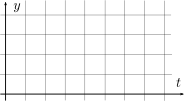
\includegraphics[scale=0.25]{lecture1_fig3.png}
\end{multicols}


}

\subsection{Euler's Method in MATLAB}
\frame[containsverbatim]{
  \frametitle{Euler's Method in MATLAB}

 \begin{lstlisting}
% approximate with Euler's forward integration
v_eu(1)=v0;
for j=1:length(time)-1
    v_eu(j+1)=v_eu(j)+(f(time(j),v_eu(j),m,c))*dt;  
end

% If this is an 'Inline Definition' of the function 
% it MUST go at the bottom of the script
function [dvdt]=f(t,v,M,C)
    dvdt=-C/M*v;
end

  \end{lstlisting}

}

% Section 2 - A More Exciting Model
\section{A More Exciting Model}
\subsection{A More Exciting Model}
\frame{

\frametitle{A More Exciting Model}
\begin{itemize}

\item First and second order linear models are frequently used  in science and engineering

\item However the world is \underline{\hspace{15mm}-\hspace{40mm}}\\

\item Many exciting and important engineering problems invlove {\bf more complex models} involving rotational motion.

\end{itemize}

\includegraphics[scale=0.15]{ur5e.png}
\includegraphics[scale=0.25]{dji_phantom.jpg}
\includegraphics[scale=0.07]{steady_cam.jpg}

}

\frame{

\frametitle{Non-Linear Swinging Pendulum}

An example of a non-linear system is an {\it inverted pendulum metronome}. \vspc

\begin{multicols}{2}
\includegraphics[scale=0.15]{metronome.png}

How will this system behave?\vspc
\scalebox{1}{$I_o\ddot{\theta}+k_T-\left( m\cdot g\cdot l\right) sin(\theta)=0$} \vspcc

Finding an analytical solution is {\bf very involved} and only mathematicians have time for all that...but you can look \href{https://www.researchgate.net/publication/230969993_A_comprehensive_analytical_solution_of_the_nonlinear_pendulum}{\color{blue}here\color{black}}

\end{multicols}

}

% Section 3 - Equation Decomposition
\section{Equation Decomposition}
\subsection{Equation Decomposition}
\frame{
As we have seen using Euler's method is not hard, but we have to setup the problem correctly. This is a reoccuring theme! \vspccc
\scalebox{1}{$I_o\ddot{\theta}+k_T-\left( m\cdot g\cdot l\right) sin(\theta)=0$} \vspcc

To solve a second order system with an integration method like Euler's you must write the {\bf slope function(s)}. \vspccc

There are two derivatives so there are two \underline{\hspace{15mm}}\hspace{3mm}\underline{\hspace{20mm}}. \vspc

}


\subsection{x2 First Order from x1 Second Order}
\frame{

\frametitle{x2 First Order from x1 Second Order}

{\it One} second order ODE can be {\bf decomposed} into {\it two} first order ODEs through a simple change of variables. This step can be confusing, but remember it is just an algebraic substitution!\vspccc

	\scalebox{1}{$I_o\ddot{\theta}+k_T-\left( m\cdot g\cdot l\right) sin(\theta)=0$} \vspcc 


}


\subsection{The Slope Function}
\frame{

\frametitle{The Slope Function}

The differential equation must be written as a function describing the first derivative or {\bf the slope} of the dependent variable.\vspc

	\scalebox{1.25}{$f(x,y)=\frac{rise}{run}=\frac{dy}{dx}\neq y(x)$}\vspcc
	or with subscript notation shown below\vspcc
	\scalebox{1.25}{$f(x_i,y_i)$}\vspcc
	

\small Careful: The first argument $x$ is not always used and is often left out. However it is an important placeholder (ODE45()) and shows this method can be used for {\it non-linear} equations with generalized input functions. 

}

\subsection{Forward Integration}
\frame{

\frametitle{Forward Integration}

Using this concept to solve the initial value problem is called {\bf Euler's forward integration} or {\bf Euler's Method}. Most of the time, the independent variable is \underline{\hspace{30mm}}. \vspcc

Compute the values of the solution one-by-one {\bf forward in time}. \vspcc
\begin{multicols}{2}
\scalebox{1}{$\underline{y(t_{i+1})=y(t_i)+f(t_i,y_i)\Delta t}$}\vspc
\scalebox{1}{$y(\hspccc)=y(\hspccc)+f(\hspccc,\hspccc)\Delta t$}\vspc
\scalebox{1}{$y(\hspccc)=y(\hspccc)+f(\hspccc,\hspccc)\Delta t$}\vspc
\scalebox{1}{$y(\hspccc)=y(\hspccc)+f(\hspccc,\hspccc)\Delta t$}\vspc

\hspace{5mm}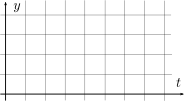
\includegraphics[scale=0.25]{lecture1_fig3.png}
\end{multicols}

}
% Section 4: A Simple Example

\section{A Simple Example}
\frame{

\frametitle{The Previous Example - Radio Flyer}

\begin{multicols}{2}
If this is a valid technique we should be able to solve the problem we solved in the previous lecture. Ferrari anyone? Let's do a Radio Flyer instead. \\ 

\hspace{10mm}\includegraphics[scale=0.15]{Radio-Flyer.jpg} \vspc

\end{multicols}

\scalebox{1.25}{$m\dot{v}+cv=0 \hspace{3mm} with \hspace{3mm}v(t=0)=v_0$} \vspcc
\scalebox{1.25}{$\hspace{5mm}\implies\hspace{5mm}v(t)=v_0e^{-\frac{c}{m}t}$} \vspace{5mm}\\

}


\frame{

\subsection{The Problem Statement}
\frametitle{The Problem Statement}

This method is not difficult {\it if} we setup  the problem correctly. Read the problem statement carefully.\vspcc

\begin{framed}
Approximate a solution to the differential equation using Euler's Method. Graph the solution from $0$ to $10$ seconds and use a stepsize of $\Delta t=\paramDTA,\hspc\paramDTA,\hspc$and$\hspc \paramDTA $ seconds.\vspcc
\scalebox{1.25}{$m\dot{v}+cv=0 \hspace{3mm} with \hspace{3mm}v(t=0)=v_0$}\vspcc
\scalebox{1.0}{$m=\paramM(kg), \hspc c=\paramC (\frac{n-m}{s}), v_0=\paramVO(\frac{m}{s})$}
\end{framed}

}

\frame{


\frametitle{Breakdown The Problem Statement}
\begin{tabular}{cc}
\underline{ODE:}&\scalebox{1.0}{$m\dot{v}+cv=0$}\vspcc
\underline{Initial Condition:}&\scalebox{1.0}{$\hspace{3mm}v(t=0)=v_0$}\vspcc
\underline{Parameters:}&\scalebox{1.0}{$m=100(kg), \hspc c=0.5 (\frac{n-m}{s}), v_0=5(\frac{m}{s})$}\vspcc
\underline{Strategy:}& Euler's Method, $\Delta t=\paramDTA,\hspc\paramDTB,\hspc$and$\hspc \paramDTC (s) $  \vspccc
\end{tabular}

Look at the formula we derived. What goes where?\vspcc


\scalebox{1.0}{$y_{i+1}=y_i + f(x_i,y_i)\Delta x$}\vspcc
}




\subsection{Execute Euler's Method}

\frame{
\frametitle{Execute Euler's Method}
First, write the {\bf slope function}. \vspc
\scalebox{1}{$f(t,y(t))=f(t,y)=$}\vspc
Then, start with the initial condition and compute the values of the solution {\it one by one, forward in time}. \vspcc

\scalebox{1}{$\underline{v(t_{i+1})=v(t_i)+f(v(t_i))\Delta t}$}\vspc
\scalebox{1}{$v(\hspccc)=v(\hspccc)+f(\hspccc)\Delta t$}\vspc
\scalebox{1}{$v(\hspccc)=v(\hspccc)+f(\hspccc)\Delta t$}\vspc
\scalebox{1}{$v(\hspccc)=v(\hspccc)+f(\hspccc)\Delta t$}\vspc
\scalebox{1}{$v(\hspccc)=v(\hspccc)+f(\hspccc)\Delta t$}\vspc

 This method is not suitable for manual computation. \vspace{0mm}\\

}


% Section 4: MATLAB Solution
\section{MATLAB Solution}

\subsection{Part 1 - Setup and Analytical Solution}
\frame[containsverbatim]{
  \frametitle{Part 1 - Setup and Analytical Solution}



\begin{lstlisting}
% ME 3001 - Mechanical Engineering Analysis
% Tristan Hill - Spring 2020
% Numerical Integration - Lecture 1 
clear variables;close all;clc

% define the constant parameters
m=100;c=1.5;v0=2.0;
dt=1.0;tstop=60;

% create an array of time values
time=0:dt:tstop;
% compute solution from derived equation
v_exact=v0*exp(-c/m*time);
\end{lstlisting}

}

\subsection{Part 2 - Euler's Method}
\frame[containsverbatim]{
  \frametitle{Part 2 - Euler's Method}

% This method is not suitable for manual computation. \vspace{0mm}\\

 \begin{lstlisting}
% approximate with Euler's forward integration
v_eu(1)=v0;
for j=1:length(time)-1
    v_eu(j+1)=v_eu(j)+(f(time(j),v_eu(j),m,c))*dt;  
end

% If this is an 'Inline Definition' of the function 
% it MUST go at the bottom of the script
function [dvdt]=f(t,v,M,C)
    dvdt=-C/M*v;
end

  \end{lstlisting}

}

\subsection{Part 3 - Graph the Solutions}
\frame[containsverbatim]{
  \frametitle{Part 3 - Graph the Solutions}

% This method is not suitable for manual computation. \vspace{0mm}\\

 \begin{lstlisting}
% plot the results of both methods
figure(1);hold on
plot(time,v_exact,'r-','LineWidth',2)
plot(time,v_eu,'b*')

% add some labels
title('Radio Flyer: mdv/dt+cv=0, v(t=0)=v0')
legend('Exact','Euler''s')
xlabel('Time (s)')
ylabel('Velocity')
grid on
  \end{lstlisting}

}


\frame[containsverbatim]{
\frametitle{ Do you believe the results?}

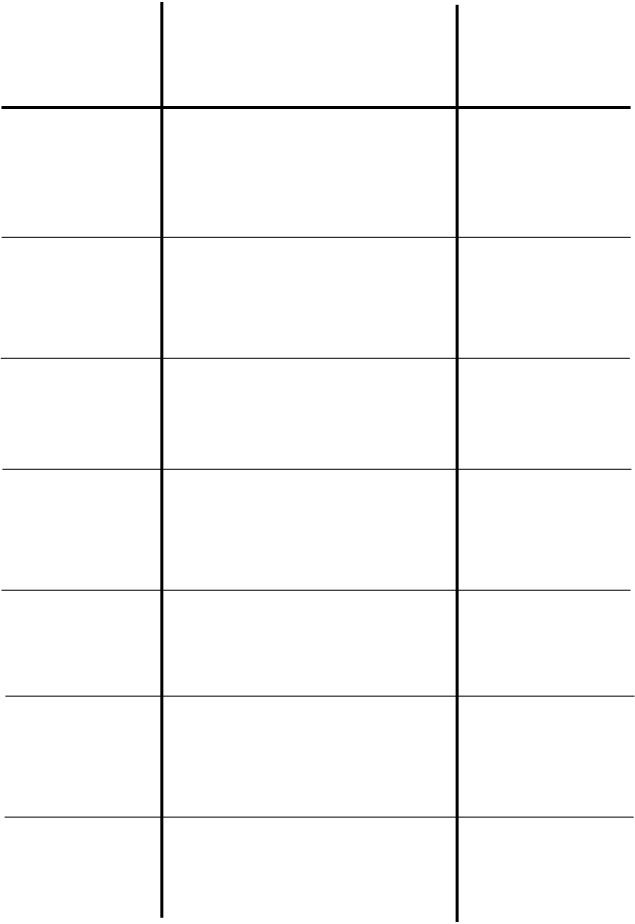
\includegraphics[scale=0.35]{lecture1_fig4.png} \vspc


}


\end{document}









